It's interesting to note that many (all?) supervised NLP tasks can be framed as question answering. Question answering is a specific type of problem in which the model is given an input text and a question about it, and is expected to produce an answer. Traditionally this might mean extracting some factual information from the input text (e.g. input: ``John ate a green apple." question: ``What color was the apple?" answer: ``green"). However, other tasks can also be framed as question answering, e.g. sentiment analysis (``What is the sentiment?"), coreference resolution (``Who does `she' refer to?), machine translation (``What is this sentence in French?"), part-of-speech tagging (``What is the POS of each word in this sentence?"), and named entity recognition (``What are all the named entities in this sentence?").

It could thus be very valuable to build a single model for general question answering. However, as of 2015-2016 there were a couple of obstacles to this in today's world:
\begin{itemize}
\item There wasn't a single architecture that consistently achieves state-of-the-art results across many tasks. Each task had a different state-of-the-art model.
\item Fully joint multitask learning (i.e. not just transfer learning/fine-tuning, but actually sharing the same weights) is difficult. Usually multi-task learning is restricted to the lower (farther from the output) layers of a model, and is only successful when the tasks are closely related (performance usually suffers if the tasks are unrelated).
\end{itemize}

The Dynamic Memory Network (\begin{tt}https://arxiv.org/abs/1506.07285\end{tt}) set out to tackle the first obstacle.

\subsection{Dynamic Memory Networks}
The core idea behind Dynamic Memory Networks (DMNs) was that it's easier to answer questions about the input text if the model is able to refer back to it, rather than forcing the model to do a pass over the input and memorize the whole thing. It consists of multiple modules that each handle a specific part of the task. Figure \ref{dmn_arch} gives a graphical overview of the different modules and how they interact, described below:
\begin{itemize}
\item The semantic memory module (not shown in the figure) simply stores word embeddings. The input and question modules refer to this when operating over the input and question text, respectively.
\item The input module is some RNN structure (in the case of this paper, a GRU) that reads over the input text. 
\begin{itemize}
\item When the input text is a single sentence, this module outputs the recursive hidden state at each time step. When it is multiple sentences, the module puts delimiter tokens between the sentences and outputs the hidden state at the end of every sentence. Let $c$ represent the outputs of the input module, and $c_i$ represent the $i$-th item of $c$.
\item A later paper found that it was helpful to use two GRUs, one left-to-right and one right-to-left, and sum the representations of the two GRUs.
\end{itemize}
\item The question module is some RNN structure (also a GRU in the paper) that reads over the question text and outputs its final hidden state $q$.
\item The episodic memory module is the most involved. It is a series of $T_M$ modified GRUs, in which each one attends to $c$, using the final hidden state of the previous GRU and $q$ as the attention input. (The first GRU only uses $q$ to perform attention.) This will be explained in greater detail in a later section. It produces a final input $m^{T_M}$.
\item The answer module uses $M^{T_M}$ to generate an answer. It is also a GRU, which at each time step takes in the output of the previous timestep $y^{t-1}$ concatenated with the question module's output $q$, and produces a new hidden state $a^t$ using those and the previous hidden state. An output is calculated at each time step using a simple matrix multiplication and softmax on the hidden state. Mathematically:
$$a_t = \text{GRU}\left(\left[y_{t-1}; q\right], a_{t-1}\right),\quad y_t = \text{softmax}\left(W^{(a)}a_t\right)$$, where $[;]$ denotes concatenation.
\end{itemize}

\begin{figure} 
\centering
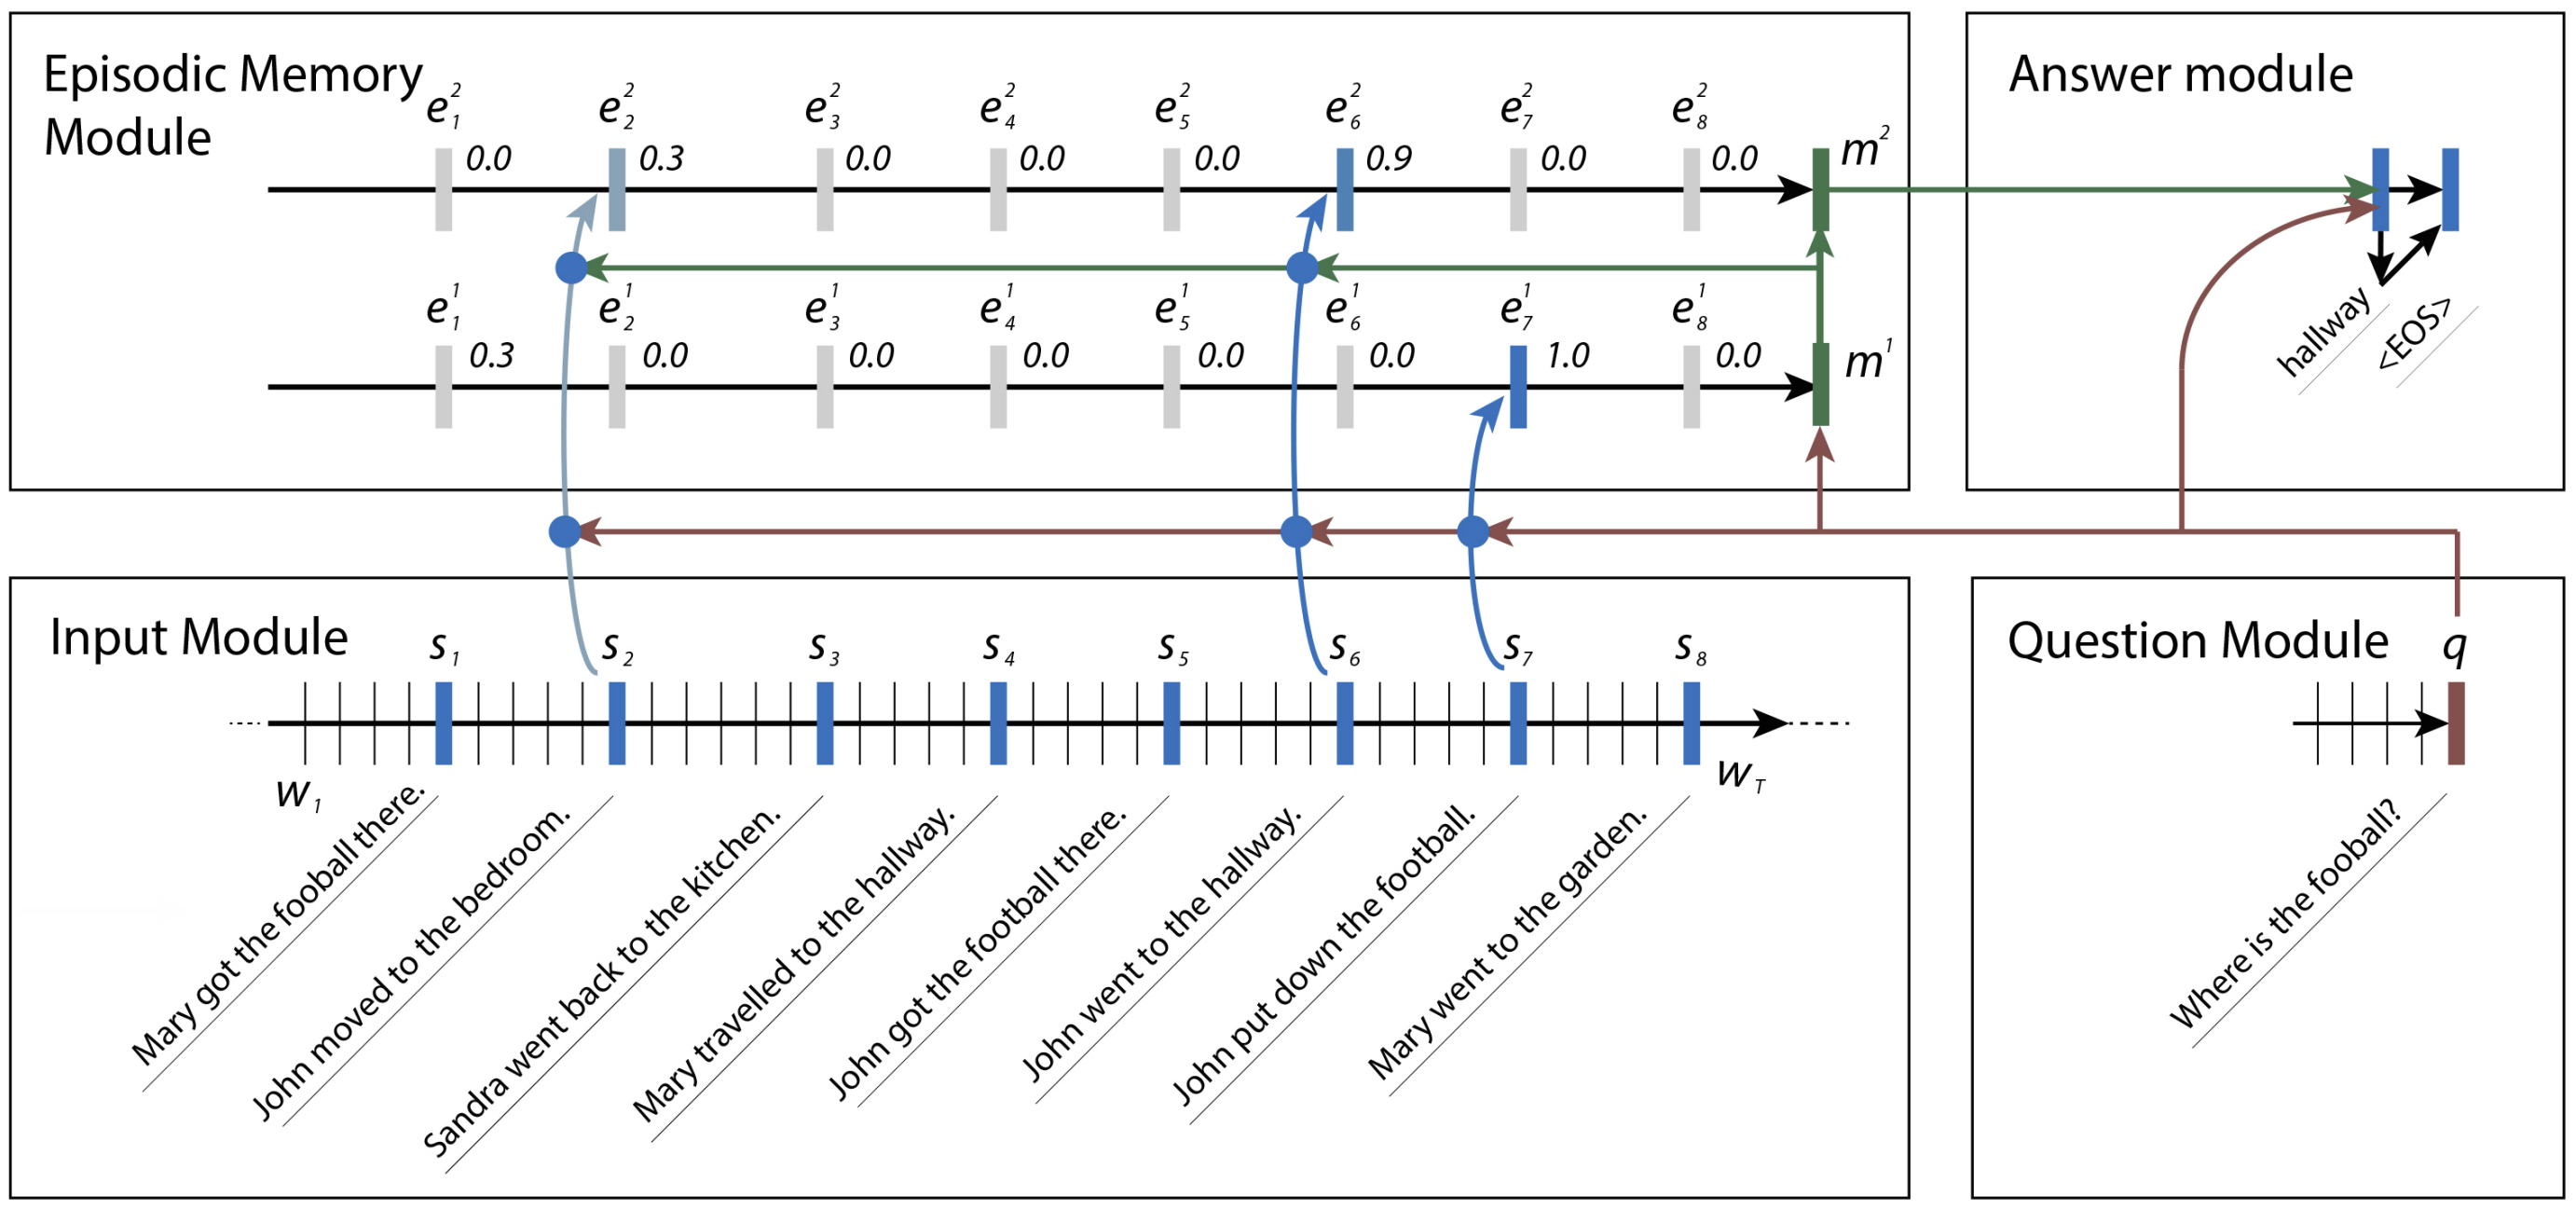
\includegraphics[scale=0.3]{dmn_arch.png}
\caption{The various modules of the DMN. The semantic memory module is not shown, but conceptually it feeds into the input module.}\label{dmn_arch}
\end{figure}

\subsubsection{Episodic memory module}
As mentioned earlier, the episodic memory module consists of a series of modified GRUs, each one attending over the input module's output using the final hidden state of the previous GRU and the question mo. The number of these stacked GRUs (each one essentially being another pass over the input) can either be fixed, or you can use a classifier at the end of each one to decide whether to do another pass.

The main mechanism of the GRU is governed by the following equation:
$$h_i^t = g_i^t\text{GRU}\left(c_i, h_{i-1}^t\right) + (1 - g_i^t)h_{i-1}^t,$$
where $t$ represents which pass over the input we're on, $i$ represents the position in the sequence, $c_i$ is the $i$-th item in the input module's output, $h_i^t$ represents the hidden units, and $g_i^t$ represents the attention mechanism. $g_i^t$ is calculated as:
\begin{align*}
z_i^t &= \left[c_i \circ q; c_i \circ m^{t-1}; \left| c_i - q\right|; \left| c_i - m^{t-1}\right|\right]\\
Z_i^t &= W^{(2)}\tanh\left(W^{(1)}z_i^t + b^{(1)}\right) + b^{(2)}\\
g_i^t &= \frac{\exp\left(Z_i^t\right)}{\sum_i \exp\left(Z_i^t\right)}\\
\end{align*}
Here $\circ$ denotes elementwise multiplication and $|x|$ denotes absolute value. $m^{t}$ denotes the final hidden state of the $t$-th GRU, $W^{(1)}$ and $W^{(2)}$ are learned weight matrices, and $b^{(1)}$ and $b^{(2)}$ are learned bias vectors. Intuitively, $g_i^t$ is activated when the current $c_i$ is determined to be important to answering the question.

A similar model to the DMN is the Memory Network (\begin{tt}https://arxiv.org/pdf/1410.3916.pdf\end{tt}). Some points of comparison:
\begin{itemize} 
\item Both have input, scoring, attention/response mechanisms.
\item MemNets use bag-of-words representation of inputs and explicitly encodes position into embeddings.
\item MemNets iteratively run many different kinds of functions, including for attention and response. (In contrast, the DMN mostly runs on GRUs.)
\end{itemize}
The papers (MemNets linked above, DMNs at beginning) offer more details.

\subsection{Results}
The model performed comparably to the existing state-of-the-art on the bAbI dataset tasks, and achieved new state-of-the-art on the Stanford Sentiment Treebank dataset (sentiment analysis) and matched the existing state-of-theart on POS tagging (WSJ-PTB dataset, on which it actually achieved new state-of-the-art by ensembling the 4 best dev-tuned models). Interestingly, the results showed that the optimal number of passes to perform over the input differed with each task (e.g. 2 for sentiment analysis and 5 for 3-fact reasoning).

It's interesting to examine some examples on the sentiment analysis dataset where the DMN predicted the wrong answer when only given one pass over the input, but got the correct answer when given two passes:
\begin{itemize}
\item ``In its ragged, cheap, and unassuming way, the movie works.” (Answer: positive, one-pass predicted negative)
\item ``The best way to hope for any chance of enjoying this film is by lowering your expectations.” (Answer: negative, one-pass predicted very positive)
\item ``The film starts out as competent but unremarkable…and gradually grows into something of considerable power.” (Answer: positive, one-pass predicted negative)
\item ``My response to the film is best described as lukewarm.” (Answer: negative, one-pass predicted positive)
\end{itemize}

For POS tagging, the model put the answer module on every sequence position, and also only performed one pass over the input.

\subsubsection{Image question answering?}
A subsequent paper (\begin{tt}https://arxiv.org/abs/1603.01417\end{tt}) replaced the input module of the DMN with a CNN that extracted features from images, and was able to achieve new state-of-the-art results on the Visual Question Answering dataset. At an extremely high level, the CNN extracted a $14\times 14$ grid of 512-dimensional feature vectors from each image and passed those into a bidirectional GRU in the input module.
